\documentclass{standalone}
\usepackage{PhysicalChemistryNote}
\begin{document}
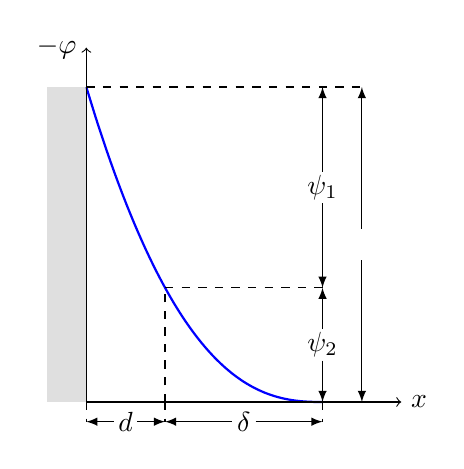
\begin{tikzpicture}
    \draw[domain=0:3,thick,blue] plot[smooth](\x,{(3-\x)^(2.5)/(3^2.5)*4});
    \draw[->] (0,0)--(4,0) node[right]{$x$};
    \draw[->] (0,0)--(0,4.5) node[left]{$-\varphi$};
    \draw[dashed] (1,0)--(1,{(2^2.5)/(3^2.5)*4});
    \draw[dashed] (0,4)--(3.5,4);
    \draw[dashed] (1,{(2^2.5)/(3^2.5)*4})--(3,{(2^2.5)/(3^2.5)*4});
    \draw[dashed] (1,0)--(1,-0.25);
    \draw[dashed] (3,0)--(3,-0.25);
    \draw[dashed] (0,0)--(0,-0.25);
    \node at (3,{(2^2.5)/(3^2.5)*2}) {$\psi_2$};
    \node at (3,{(2^2.5)/(3^2.5)*2+2}) {$\psi_1$};
    \node at (3.5,2) {$\ep$};
    \node at (0.5,-0.25) {$d$};
    \node at (2,-0.25) {$\delta$};
    \draw[-latex] (3,{(2^2.5)/(3^2.5)*2-0.2})--(3,0);
    \draw[-latex] (3,{(2^2.5)/(3^2.5)*2+0.2})--(3,{(2^2.5)/(3^2.5)*4});
    \draw[-latex] (3,{(2^2.5)/(3^2.5)*2+1.8})--(3,{(2^2.5)/(3^2.5)*4});
    \draw[-latex] (3,{(2^2.5)/(3^2.5)*2+2.2})--(3,4);
    \draw[-latex] (3.5,1.8)--(3.5,0);
    \draw[-latex] (3.5,2.2)--(3.5,4);
    \draw[-latex] (2.15,-0.25)--(3,-0.25);
    \draw[-latex] (1.85,-0.25)--(1,-0.25);
    \draw[-latex] (0.65,-0.25)--(1,-0.25);
    \draw[-latex] (0.35,-0.25)--(0,-0.25);
    \fill[lightgray,opacity=0.5] (-0.5,0)rectangle(0,4);
\end{tikzpicture}
\end{document}